\documentclass{sig-alternate-ipsn13}
\usepackage{ntheorem}
\usepackage{algorithm}
\usepackage{algorithmic}
\usepackage{todonotes}

%-----------------------------------------------------------------------------------------------------------------------------------------------------------------
% Sets
\newcommand{\Fbb}{\mathbb{F}}
\newcommand{\Rbb}{\mathbb{R}}
\newcommand{\Cbb}{\mathbb{C}}
\newcommand{\Nbb}{\mathbb{N}}
\newcommand{\Qbb}{\mathbb{Q}}
\newcommand{\Zbb}{\mathbb{Z}}

\newcommand{\Acal}{\mathcal{A}}
\newcommand{\Bcal}{\mathcal{B}}
\newcommand{\Ccal}{\mathcal{C}}
\newcommand{\Dcal}{\mathcal{D}}
\newcommand{\Ecal}{\mathcal{E}}
\newcommand{\Fcal}{\mathcal{F}}
\newcommand{\Gcal}{\mathcal{G}}
\newcommand{\Hcal}{\mathcal{H}}
\newcommand{\Ical}{\mathcal{I}}
\newcommand{\Jcal}{\mathcal{J}}
\newcommand{\Kcal}{\mathcal{K}}
\newcommand{\Lcal}{\mathcal{L}}
\newcommand{\Mcal}{\mathcal{M}}
\newcommand{\Ncal}{\mathcal{N}}
\newcommand{\Ocal}{\mathcal{O}}
\newcommand{\Pcal}{\mathcal{P}}
\newcommand{\Qcal}{\mathcal{Q}}
\newcommand{\Rcal}{\mathcal{R}}
\newcommand{\Scal}{\mathcal{S}}
\newcommand{\Tcal}{\mathcal{T}}
\newcommand{\Ucal}{\mathcal{U}}
\newcommand{\Vcal}{\mathcal{V}}
\newcommand{\Wcal}{\mathcal{W}}
\newcommand{\Xcal}{\mathcal{X}}
\newcommand{\Ycal}{\mathcal{Y}}
\newcommand{\Zcal}{\mathcal{Z}}

\newcommand{\bigO}{\Ocal}

%-----------------------------------------------------------------------------------------------------------------------------------------------------------------
% operators
\DeclareMathOperator*{\argmax}{arg\,max}
\DeclareMathOperator*{\argmin}{arg\,min}
\DeclareMathOperator*{\cart}{\times}
\DeclareMathOperator*{\card}{card}
\DeclareMathOperator*{\superset}{\supset}
\DeclareMathOperator*{\support}{support}

% calculus
\newcommand \ddt[1]{\frac{d #1}{dt}}
\newcommand \ppx[1]{\frac{\partial #1}{\partial x}}
\newcommand \ppxn[2]{\frac{\partial^{#2} #1}{\partial^{#2} x}}
\newcommand \ddtn[2]{\frac{d^{#2} #1}{dt^{#2}}}

% topology
\DeclareMathOperator*{\bd}{bd}
\DeclareMathOperator*{\osc}{osc}
\DeclareMathOperator*{\disc}{disc}
\DeclareMathOperator*{\cl}{cl}
\DeclareMathOperator*{\interior}{int}

% linear albegra
\DeclareMathOperator*{\dm}{dim}
\DeclareMathOperator*{\spn}{span}
\DeclareMathOperator*{\trace}{trace}
\DeclareMathOperator*{\Tr}{Tr}
\DeclareMathOperator*{\diag}{diag}

% probability
\DeclareMathOperator*{\cov}{cov}
\DeclareMathOperator*{\var}{var}
\DeclareMathOperator*{\Exp}{\mathbb{E}}
\newcommand\Expsq[1]{\Exp\sqbr{#1}}
\DeclareMathOperator*{\Pro}{\mathbb{P}}
\DeclareMathOperator*{\Prob}{\mathbb{P}}
\newcommand \convL[1]{\overset{L^{#1}}{\rightarrow} }
\newcommand \convP{\overset{\text{P}}{\rightarrow} }
\newcommand \convAS{\overset{\text{a.s.}}{\rightarrow} }



%convex optimization
\DeclareMathOperator*{\Co}{Co}
\DeclareMathOperator*{\conv}{conv}
\DeclareMathOperator*{\diam}{diam}

%complex
\DeclareMathOperator*{\Real}{Re}
\DeclareMathOperator*{\Imag}{Im}
\newcommand\contains{\ni}



%-----------------------------------------------------------------------------------------------------------------------------------------------------------------
% text
\newcommand{\by}{\text{ by }}
\newcommand{\pf}{\paragraph{\emph{proof}}}
\newcommand\p[1]{\paragraph{#1}}
\newcommand{\ans}{\paragraph{\emph{answer}}}
\newcommand{\subjectto}{\text{subject to}}
\newcommand\ind[1]{1_{#1}}

\newcommand\emp[1]{{\color{Red} #1}}

%-----------------------------------------------------------------------------------------------------------------------------------------------------------------
% matrices and equations

\newcommand \func[5]{
\[
\begin{aligned}
#1: #2 &\rightarrow #3 \\
#4 &\mapsto #5
\end{aligned}
\]
}

\newcommand \al[1]{\begin{align*}
#1
\end{align*}
}

\newcommand \aln[1]{\begin{align}
#1
\end{align}
}

\newcommand \ald[1]{
\[
\begin{aligned}
#1
\end{aligned}
\]
}

\newcommand \aldn[1]{
\begin{equation}
\begin{aligned}
#1
\end{aligned}
\end{equation}
}


\newcommand \mat[1]{
\left(
\begin{array}
#1
\end{array}
\right)
}

\newcommand \Det[1]{
\left|
\begin{array}
#1
\end{array}
\right|
}
%-----------------------------------------------------------------------------------------------------------------------------------------------------------------
%other
\newcommand{\horline}{
\begin{center}
\line(1,0){500}
\end{center}
}

\newcommand \vs{\vspace{40pt}}

\newcommand \imp{\Rightarrow}
\newcommand \eqv{\Leftrightarrow}



%-----------------------------------------------------------------------------------------------------------------------------------------------------------------
% parenthesis and such
\newcommand \floor[1]{\lfloor #1 \rfloor}
\newcommand \ceil[1]{\left\lceil #1 \right\rceil}
\newcommand \bra{\left\langle}
\newcommand \ket{\right\rangle}
\newcommand \braket[2]{\bra #1, #2 \ket}
\newcommand{\psh}[2]{\ensuremath{\langle #1,#2\rangle}}
\newcommand \parenth[1]{\left( #1 \right)}
\newcommand \curl[1]{\left\{ #1 \right\}}
\newcommand \sqbr[1]{\left[ #1 \right]}
\newcommand \sqbra[1]{\left[ #1 \right]}


%-----------------------------------------------------------------------------------------------------------------------------------------------------------------







%-----------------------------------------------------------------------------------------------------------------------------------------------------------------
% Algorithms
\usepackage{listings} % for algorithms
\usepackage{framed}
% setup of the lst
\lstset{ %
  basicstyle=\footnotesize,
  commentstyle=\color{gray},
  extendedchars=true,
  frame=single,
  keywordstyle=\color{blue},
  language=Java,
  morekeywords={trait, def, val},
  numbers=left,
  numbersep=5pt,
  numberstyle=\tiny\color{gray},
  tabsize=2
}




\newtheorem{remark}{Remark}
\newtheorem{theorem}{Theorem}
\newtheorem*{nonumtheorem}{Theorem}
\newtheorem{definition}{Definition}
\newtheorem{proposition}{Proposition}


% \usepackage{picins}
% \usepackage{graphicx}

% \makeatletter
% \def\Ginclude@graphics#1{%
%   \parpic(\Gin@@ewidth,\Gin@@eheight)[d]{#1}\picskip{0}}%
% \makeatother


\begin{document}

\title{Estimating Learning Dynamics in the Routing Game
% \titlenote{}
}
%
% You need the command \numberofauthors to handle the 'placement
% and alignment' of the authors beneath the title.
%
% For aesthetic reasons, we recommend 'three authors at a time'
% i.e. three 'name/affiliation blocks' be placed beneath the title.
%
% NOTE: You are NOT restricted in how many 'rows' of
% "name/affiliations" may appear. We just ask that you restrict
% the number of 'columns' to three.
%
% Because of the available 'opening page real-estate'
% we ask you to refrain from putting more than six authors
% (two rows with three columns) beneath the article title.
% More than six makes the first-page appear very cluttered indeed.
%
% Use the \alignauthor commands to handle the names
% and affiliations for an 'aesthetic maximum' of six authors.
% Add names, affiliations, addresses for
% the seventh etc. author(s) as the argument for the
% \additionalauthors command.
% These 'additional authors' will be output/set for you
% without further effort on your part as the last section in
% the body of your article BEFORE References or any Appendices.

\numberofauthors{3} %  in this sample file, there are a *total*
% of EIGHT authors. SIX appear on the 'first-page' (for formatting
% reasons) and the remaining two appear in the \additionalauthors section.
%
\author{
% You can go ahead and credit any number of authors here,
% e.g. one 'row of three' or two rows (consisting of one row of three
% and a second row of one, two or three).
%
% The command \alignauthor (no curly braces needed) should
% precede each author name, affiliation/snail-mail address and
% e-mail address. Additionally, tag each line of
% affiliation/address with \affaddr, and tag the
% e-mail address with \email.
%
% 1st. author
\alignauthor Kiet Lam\\
\affaddr{UC Berkeley}
\email{\small\texttt{kiet.lam@berkeley.edu}}
\alignauthor Walid Krichene\\
\affaddr{UC Berkeley}
\email{\small\texttt{walid@eecs.berkeley.edu}}
\alignauthor Alexandre Bayen\\
\affaddr{UC Berkeley}
\email{\small\texttt{bayen@berkeley.edu}}
% \alignauthor
% Ben Trovato\titlenote{Dr.~Trovato insisted his name be first.}\\
%        \affaddr{Institute for Clarity in Documentation}\\
%        \affaddr{1932 Wallamaloo Lane}\\
%        \affaddr{Wallamaloo, New Zealand}\\
%        \email{trovato@corporation.com}
% % 2nd. author
% \alignauthor
% G.K.M. Tobin\titlenote{The secretary disavows
% any knowledge of this author's actions.}\\
%        \affaddr{Institute for Clarity in Documentation}\\
%        \affaddr{P.O. Box 1212}\\
%        \affaddr{Dublin, Ohio 43017-6221}\\
%        \email{webmaster@marysville-ohio.com}
% % 3rd. author
% \alignauthor Lars Th{\o}rv{\"a}ld\titlenote{This author is the
% one who did all the really hard work.}\\
%        \affaddr{The Th{\o}rv{\"a}ld Group}\\
%        \affaddr{1 Th{\o}rv{\"a}ld Circle}\\
%        \affaddr{Hekla, Iceland}\\
%        \email{larst@affiliation.org}
% \and  % use '\and' if you need 'another row' of author names
% % 4th. author
% \alignauthor Lawrence P. Leipuner\\
%        \affaddr{Brookhaven Laboratories}\\
%        \affaddr{Brookhaven National Lab}\\
%        \affaddr{P.O. Box 5000}\\
%        \email{lleipuner@researchlabs.org}
% % 5th. author
% \alignauthor Sean Fogarty\\
%        \affaddr{NASA Ames Research Center}\\
%        \affaddr{Moffett Field}\\
%        \affaddr{California 94035}\\
%        \email{fogartys@amesres.org}
% % 6th. author
% \alignauthor Charles Palmer\\
%        \affaddr{Palmer Research Laboratories}\\
%        \affaddr{8600 Datapoint Drive}\\
%        \affaddr{San Antonio, Texas 78229}\\
%        \email{cpalmer@prl.com}
}
% There's nothing stopping you putting the seventh, eighth, etc.
% author on the opening page (as the 'third row') but we ask,
% for aesthetic reasons that you place these 'additional authors'
% in the \additional authors block, viz.
% \additionalauthors{Additional authors: John Smith (The Th{\o}rv{\"a}ld Group,
% email: {\texttt{jsmith@affiliation.org}}) and Julius P.~Kumquat
% (The Kumquat Consortium, email: {\texttt{jpkumquat@consortium.net}}).}
% \date{30 July 1999}
% Just remember to make sure that the TOTAL number of authors
% is the number that will appear on the first page PLUS the
% number that will appear in the \additionalauthors section.

\maketitle
\begin{abstract}
  The routing game models congestion on transportation and communication networks.
  We consider an online learning model of player dynamics: at each iteration, every player chooses a route (or a probability distribution over routes), then the joint decision of all players determines the costs of each path, which are then revealed to the players. We first review convergence guarantees of such online learning dynamics. Then, we consider the following estimation problem: given a sequence of player decisions and the corresponding costs, we would like to fit the learning model parameters to these observations. We consider in particular entropic mirror descent dynamics, and develop a numerical solution to the estimation problem.

  We demonstrate this method using data collected from a routing game experiment: we develop a web interface to simulate the routing game. When players log in to the interface, they are assigned an origin and destination on the graph. They can choose, at each iteration, a distribution over their available routes, and each player seeks to minimize her own cost. We collect a data set using this interface, then we apply the proposed method to fit the learning model parameters.
  We observe in particular that after an exploration phase, the joint decision of the players remains within a small distance of the Nash equilibrium. We also use the estimated model parameters to predict the flow distribution over routes, and compare these predictions to the actual distribution.
  Finally, we discuss some of the qualitative implications of the experiment, and give directions for future research.

\end{abstract}

%============================================================================================
\section{Introduction}
The routing game is a non-cooperative game that models congestion in transportation and communication networks. The game is given by a directed graph that represents the network, and each player is given by a source node and destination node, and seeks to send traffic (either packets in a communication setting, or cars in a  transportation setting) while minimizing the total delay of that traffic. The delay is determined by the joint decision of all players, such that whenever an edge has high load, it becomes congested and any traffic using that edge incurs additional delay.

This model of congestion is simple yet powerful, and routing games have been studied extensively since the seminal work of Beckman~\cite{beckmann1955studies}. The Nash equilibria of the game are simple to characterize, and have been used to quantify the inefficiency of the network, using the price of anarchy~\cite{roughgarden2002bad}. However, the Nash equilibrium concept may not offer a good descriptive model of actual behavior of players, as argued by many authors, including for example~\cite{fox2013population}. Besides the assumption of rationality, which can be questioned, the Nash equilibrium assumes that players have a complete description of the structure of the game, their own cost functions, and those of other players. This model is arguably not very realistic for the routing game, as one does not expect users of a network to have an accurate representation of the cost function on every edge of the network, or of the other users of the network.
One alternative to the Nash equilibrium concept is a model of repeated play, sometimes called learning models or adjustment models. In such models, one assumes that each player makes decisions iteratively, and uses the outcome of each iteration to adjust their next decision. Formally, if $x_k^{(t)}$ is the decision of player $k$ at iteration $t$, and $\ell^{(t)}_k$ is the corresponding vector of costs, then player $k$ faces a sequential decision problem in which she chooses $x^{(t)}_k$ then observes $\ell_k^{(t)}$. These sequential decision problems are coupled through the cost functions, since $\ell_k^{(t)}$ depends not only on $x_k^{(t)}$ but also on $x_{k'}^{(t)}$ for $k' \neq k$ (but players do not necessarily model this coupling). Such models have a long history in game theory, and date back to the work of Hannan~\cite{hannan1957approximations} and Blackwell~\cite{blackwell1956analog}. In recent years, there has been a resurgence of research on the topic of learning in games using sequential decision problems, see for example~\cite{cesa2006prediction} and the references therein.

When designing a model of player decisions, many properties are desirable. Perhaps the most important property is that the dynamics should be consistent with the equilibrium of the game, in the following sense: asymptotically, one should expect the learning dynamics to converge to the equilibrium of the full information, one-shot game (be it Nash equilibrium or other, more general equilibrium concepts). In this sense, players ``learn'' the equilibrium asymptotically. Much progress has been made in recent years in characterizing classes of learning dynamics which are guaranteed to converge to an equilibrium set~\cite{freund1999adaptive, hart2001general, hart2005adaptive, fox2013population}. In particular for the routing game, different models of learning have been studied for example in~\cite{fischer2004evolution,blum2006routing,kleinberg2009multiplicative,krichene2015learning,krichene2015SMD}.

In this paper, we briefly review some of the known models of learning in the routing game. We focus in particular on the mirror descent model used in~\cite{krichene2015MD}. This model describes the learning dynamics as solving, at each step, a simple minimization problem parameterized by a learning rate $\eta$. Formally, the decision at iteration $t+1$ is obtained by solving
\[
x^{(t+1)}_k(\eta^{(t)}_k) = \argmin_{x_k \in \Delta^{\Acal_k}} \eta^{(t)}_k\braket{\ell^{(t)}_k}{x} + D_{\psi_k}(x_k, x^{(t)}_k),
\]
where $\psi_k$ is a distance generating function with corresponding Bregman divergence $D_{\psi_k}$, and $\eta^{(t)}_k$ is a learning rate. The model is reviewed in detail in Section~\ref{sec:model}. Intuitively, minimizing the first term $\braket{\ell^{(t)}_k}{x}$ will assign traffic to the routes which currently have minimal cost, and minimizing the second term $D_{\psi_k}(x_k, x^{(t)}_k)$ will keep the traffic assignment at its current value. Minimizing the linear combination trades-off both terms, and the learning rate $\eta_k^{(t)}$ determines how aggressive the player is when updating her strategy: a small learning rate results in a small change in strategy (i.e. $x^{(t+1)}_k$ is close to $x_k^{(t)}$), while a large learning rate results in a significant change.

Motivated by this interpretation of learning rates, we propose in Section~\ref{sec:estimation}, the following estimation problem: given a sequence of player decisions $(x^{(t)}_k)$, and the sequence of corresponding losses $(\ell_k^{(t)})$, can we fit a learning model to these observations? A simple approach is to assume that the player is using a given distance generating function $\psi_k$, and estimate $\eta_k$ for example by minimizing the distance between the observed decision $\bar x^{(t+1)}_k$, and the decision predicted by the model, $x^{(t+1)}_k(\eta_k)$. More precisely, we can choose $\eta^{(t)}_k$ to minimize $D_{\psi_k}(\bar x^{(t+1)}_k, x^{(t+1)}_k(\eta))$. We show that in the entropic case (when $\psi_k$ is the negative entropy), this problem is convex, thus $\eta_k^{(t)}$ can be estimated efficiently e.g. by using gradient descent. This method allows us to estimate one parameter $\eta_k^{(t)}$ per iteration $t$. When we have a sequence of observations available, it can be desirable to control the complexity of the model by assuming a parameterized sequence of learning rates, instead of estimating each term separately. Thus, we propose a second method which assumes that the learning rate is of the form $\eta^{(t)}_k = \eta^{(0)}_k t^{-\alpha_k}$, with $\alpha_k \in (0, 1)$. The resulting estimation problem is non-convex in general, but since it is a two dimensional problem, it can be solved efficiently. Finally, we consider a family of distance generating functions $\psi_\epsilon$, parameterized by $\epsilon$, that can be viewed as a generalization of the negative entropy function. These generalized entropy functions also offer some desirable properties that we discuss in Section~\ref{sec:estimation}. We also briefly discuss potential uses for the estimated model: for example, the model can be used simply to predict the decision of the players over the next few iterations, by propagating the model forward with the estimated values of the parameters; more generally, the model can be used to formulate a receding-horizon optimal control problem, by using the current estimate of the model as a plant in the control problem.

In the second part of the paper, we present an experimental setting which we developed to collect data on routing decisions. We developed a web interface in which a master user can create an instance of the routing game by defining a graph and cost functions on edges of the graph. Then other users can connect to the interface as players. The game then proceeds similarly to our learning model: at each iteration, every player chooses a flow distribution on their available routes (using a graphical user interface with sliders), then their decisions are sent to a backend server, which computes the total cost of each route, and sends back this information to each player. In Section~\ref{sec:experiment}, we describe the experimental setting, some implementation details, as well as the nature of the collected data. We then use this data to run the estimation tasks which were proposed in Section~\ref{sec:estimation}, and give some qualitative and quantitative insights into the behavior of players. In particular, we observed that in the first few iterations, the flow distributions oscillate, which corresponds to a high value of estimated learning rates. For later iterations, the flow distributions are, in general, close to equilibrium, and the learning rates are lower, although some players may occasionally move the system away from equilibrium by performing an aggressive update (corresponding to a high learning rate). It is also interesting to observe that in some rare cases, the estimate of the learning rate is negative, which means that the player updated her strategy by assigning more traffic to routes with higher cost, a counter-intuitive behavior which is hard to model. We also solve the decay rate estimation problem and compare the decay rates of the different players, then use the estimated parameters to predict the traffic assignment over the next few iterations, and comment on the quality of the prediction. We conclude in Section~\ref{sec:conclusion} by summarizing our results and giving directions for future research.

%============================================================================================
\section{The routing game and the learning model}
\label{sec:model}
In this section, we give the definition of the (one-shot) routing game, and the model of learning dynamics.

\subsection{The routing game}
\label{sec:routing_game}
The routing game is played on a directed graph $\Gcal = (V, E)$, where $V$ is a vertex set and $E \subset V \times V$ is an edge set. The players will be indexed by $k \in \{1, \dots, K\}$, where every player is given by an origin vertex $o_k \in V$, a destination vertex $d_k \in V$, and a traffic mass $m_k \geq 0$ that represents the total traffic that the player needs to send from $o_k$ to $d_k$. The set of available paths connecting $o_k$ to $d_k$ will be denoted by $\Pcal_k$, and the action set of player $k$ is simply the probability simplex over $\Pcal_k$, which we denote by $\Delta_k = \{x \in \Rbb_+^{\Pcal_k} : \sum_{p \in \Pcal_k} x_p = 1\}$. In other words, each player chooses a distribution over their available paths, and their traffic is allocated to paths according to that distribution. We will denote by $x_k\in \Delta^{\Pcal_k}$ the distribution of player $k$. Note that $x_k$ is a distribution vector, so the vector of actual flows is the scaled vector $m_k x_k$. The joint decision of all players is denoted by $x = (x_1, \dots, x_K)$. The costs of the players are then determined as follows:
\begin{itemize}
\item The cost on an edge $e$ is $c_e(\phi_e(x))$, where $c_e(\cdot)$ is a given, increasing function, and $\phi_e(x)$ is the total traffic flow on edge $e$ induced by the distribution $x$, obtained simply by summing all the path flows that go through that edge, i.e. $\phi_e(x) = \sum_k \sum_{p \in \Pcal_k} m_k x_{k, p}$.
\item The cost on a path $p \in \Pcal_k$ is denoted by $\ell_{k, p}(x)$, and is the sum of edge costs along the path, i.e. $\ell_{k, p}(x) = \sum_{e \in p} c_e(\phi_e(x))$.
\item The cost for player $k$ is the total path cost for all the traffic sent by player $k$, i.e. $\sum_{p \in \Pcal_k} m_k x_{k, p} \ell_{k, p}(x)$. This is simply the inner product between the flow vector $m_k x_k$ and the path loss vector $\ell_k(x)$, which we denote by $\braket{\ell_k(x)}{x_k}$.
\end{itemize}
\begin{remark}[A note on the player model] Some formulations of the routing game, e.g.~\cite{sandholm2001potential,krichene2015learning}, formulate the game in terms of populations of players, such that each population is an infinite set of players with the same origin and destination. This assumes that each player contributes an infinitesimal amount of flow, so each player can pick a single path. In our model, each player is macroscopic, and can split its traffic across multiple routes. Both models are equivalent in terms of analysis, the only difference is in terms of interpretation of the model. We choose the finite player interpretation because it is more consistent with the experimental section of the paper, where we run the game with finitely many players.
\end{remark}

%-----------------------------------------------------------------------------------------------------------------------------------------------------------------
\begin{definition}[Nash equilibrium]
A distribution $x^\star = (x_1^\star, \dots, x_K^\star)$ is a Nash equilibrium if it satisfies the following condition: for all other distributions $x = (x_1, \dots, x_K)$ and for all~$k$,
\[
\braket{\ell_k(x^\star)}{x_k - x_k^\star} \geq 0.
\]
\end{definition}
In words, $x^\star$ is a Nash equilibrium if for every player $k$, the expected cost under $x_k^\star$ is lower than the expected cost under any other distribution $x_k$. If we define the inner product $\braket{x}{\ell} = \sum_{k} \braket{x_k}{\ell_k}$, then this is equivalent to: $x^\star$ is an equilibrium if and only if $\braket{\ell(x^\star)}{x - x^\star} \geq 0$ for all feasible $x$. This variational inequality is, in fact, equivalent to the first-order optimality condition of the following potential function, usually referred to as the Rosenthal potential, in reference to~\cite{rosenthal1973class}:
\begin{proposition}[Rosenthal potential]
Consider a routing game and define the following function
\[
f(x) = \sum_{e \in E} \int_0^{\phi_e(x)} c_e(u)du.
\]
Then $f$ is convex its gradient is $\nabla f(x) = \ell(x)$.
\end{proposition}
This result can be found for example in~\cite{roughgarden2002bad}. Due to the fact that the loss function $\ell(\cdot)$ coincides with the gradient field $\nabla f(\cdot)$ of the Rosenthal potential, the Nash condition can be rewritten as
\[
\braket{\nabla f(x^\star)}{x - x^\star} \geq 0 \ \forall \text{ feasible }x,
\]
and since $f$ is convex, this is a necessary and sufficient condition for optimality of $x^\star$ (see e.g. Section 4.2.3 in~\cite{boyd2010convex}). Therefore the set of Nash equilibria is exactly the set of minimizers of the convex potential~$f$. This is important both for computation (computing a Nash equilibrium can be done by minimizing a convex function), and for modeling: one can model player dynamics as performing a distributed optimization of the potential function. More precisely, if we adopt the point of view presented in the introduction, wherein each player faces a sequential decision problem, and plays $x^{(t)}_k$ then observes $\ell_k(x^{(t)})$, then this corresponds to a first-order distributed optimization of the function~$f$, where each player is responsible for updating the variables $x_k^{(t)}$, and observes, at each iteration, the partial gradient $\ell_k(x^{(t)}) = \nabla_{x_k} f(x^{(t)})$. Using this connection to distributed optimization, a model of player dynamics was proposed in~\cite{krichene2015MD}. We review the model in the next Section.


%-----------------------------------------------------------------------------------------------------------------------------------------------------------------
\subsection{The learning model: mirror descent dynamics}
\label{sec:learning}
We will consider the model of distributed learning proposed in~\cite{krichene2015MD}. Each player is assumed to perform a mirror descent update given by the following algorithm:
\begin{algorithm}[H]
\begin{algorithmic}
\FOR{each $t \in \{1, 2, \dots \}$}
\STATE Play $x^{(t)}_k$,
\STATE Observe $\ell_k^{(t)} = \nabla_{x_k} f(x^{(t)})$,
\STATE Update
\begin{equation}
x^{(t+1)}_k = \argmin_{x_k \in \Delta^{\Pcal_k}} \eta_k^{(t)} \braket{\ell_k(x^{(t)})}{x_k} + D_{\psi_k}(x_k, x^{(t)}_k)
\label{eq:MD_update}
\end{equation}
\ENDFOR
\end{algorithmic}
\caption{Distributed mirror descent dynamics with distance generating function $\psi_k$ and learning rates $\eta_k^{(t)}$.}
\label{alg:MD}
\end{algorithm}
In the update equation~\eqref{eq:MD_update}, $D_{\psi_k}(x, x^{(t)}_k)$ is the Bregman divergence between the distributions $x_k$ and $x_k^{(t)}$, defined as follows: $D_\psi(x, y) = \psi(x) - \psi(y) - \braket{\nabla \psi(y)}{x - y}$, for a strongly convex function $\psi$, called the distance generating function. Some special cases include
\begin{itemize}
\item The Euclidean case: if $\psi(x) = \frac{1}{2}\|x\|^2_2$, then $D_\psi(x, y) = \frac{1}{2}\|x - y\|_2^2$. In this case, mirror descent reduces to the projected gradient descent algorithm.
\item The entropic case: if $\psi(x) = - H(x)$ where $H(x) = -\sum_{p} x_p \ln x_p$ is the negative entropy, then $D_\psi(x, y) = \sum_p x_p \ln \frac{x_p}{y_p}$ is the Kullback-Leibler divergence from $x$ to $y$. In this case, the mirror descent algorithm is sometimes called the entropic descent~\cite{beck2003mirror}, or exponentiated gradient descent~\cite{kivinen1997exponentiated}.
\end{itemize}
The mirror descent method is a general method for convex optimization proposed in~\cite{nemirovski1983problem}. The model in Algorithm~\ref{alg:MD} is a distributed version of mirror descent, applied to the potential function $f$. To give some intuition of the method, the first term $\braket{\ell_k^{(t)}}{x_k}$ in the minimization problem~\eqref{eq:MD_update} can be thought of as a linear approximation of the potential function (since $\ell(x) = \nabla f(x)$), and the second term $D_\psi(x_k, x^{(t)}_k)$ penalizes deviations from the previous iterate. The learning rate $\eta_k^{(t)}$ determines the tradeoff between the two terms, and can be thought of as a generalized step size: a smaller $\eta_k$ results in a distribution which is closer to the current $x_k^{(t)}$. Thus, from the potential function point of view, the player minimizes a linearization of the potential plus a Bregman divergence term that keeps $x_k$ close to $x_k^{(t)}$. From the routing game point of view, the first term $\braket{\ell^{(t)}_k}{x_k}$ corresponds to putting weight on the paths that have smaller cost during the previous iteration, and the second term keeps the distribution at its current value.

The convergence of this distributed learning model is discussed in~\cite{krichene2015MD}. In particular, the learning dynamics is guaranteed to converge under the following assumptions:
\begin{theorem}[Theorem~3 in~\cite{krichene2015MD}]
\label{thm:convergence}
Consider the routing game with mirror descent dynamics defined in Algorithm~\ref{alg:MD}, and suppose that for all $k$, $\eta_k^{(t)}$ is decreasing and converges to $0$. Then $f(x^{(t)}) - f^\star = \Ocal\parenth{\sum_k \frac{1}{t\eta_k^{(t)}} + \frac{\sum_{\tau = 1}^t \eta_k^{(\tau)}}{t} }$.
\end{theorem}

In particular, if $\eta_k^{(t)} = \eta^{(0)}_k t^{-\alpha_k}$, with $\alpha_k \in (0, 1)$, then one can bound the sum $\sum_{\tau = 1}^t \eta_k^{(t)} = \eta^{(0)}_k \sum_{\tau = 1}^t \tau^{-\alpha_k} \leq \eta^{(0)}_k \int_0^t \tau^{-\alpha_k} d\tau = \frac{\eta^{(0)}_k}{1-\alpha_k} t^{1-\alpha_k}$. Therefore, $f(x^{(t)}) - f^\star = \Ocal(t^{\alpha_k - 1}) + \Ocal(t^{-\alpha_k}) = \Ocal(t^{-\min(\alpha_k, 1-\alpha_k)})$.

While the specific convergence rate does not matter for the purposes of the estimation problem, the convergence guarantees for decaying learning rates motivates some of the modeling assumptions made in the next Section. To conclude this Section, we also point that a stochastic version of the distributed mirror descent dynamics has been proposed and studied in~\cite{krichene2015SMD}. In that model, instead of observing the true loss vector $\ell^{(t)}_k$, a player observes a stochastic vector $\hat \ell^{(t)}_k$, the expectation of which (conditioned on all past information) is a.s. the true loss vector. A convergence result similar to Theorem~\ref{thm:convergence} is obtained, but the convergence rate is that of $\Exp[f(x^{(t)})] - f^\star$. This results is important, as it shows that convergence is robust to noise and other stochastic perturbations. For a more detailed discussion, see~\cite{krichene2015SMD}.

%============================================================================================
\section{Learning model estimation}
\label{sec:estimation}
In this section, we assume that we have access to a sequence of observations of traffic distributions $(\bar x^{(t)}_k)$, and a sequence of loss vectors $(\bar \ell^{(t)}_k)$. We use the over bar to make a clear distinction between quantities which are observed and quantities which are estimated. Given this sequence of observations, we would like to fit a model of learning dynamics. From the previous section, the learning model in Algorithm~\ref{alg:MD} is naturally parameterized by the distance generating function $\psi_k$ and the learning rate sequence $\eta_k^{(t)}$. First, we discuss how one can estimate a single term of the learning rate sequence, given a distance generating function $\psi_k$.

%-----------------------------------------------------------------------------------------------------------------------------------------------------------------
\subsection{Estimating a single learning rate}
Given the current flow distribution $\bar x^{(t)}_k$ and the current loss vector $\bar \ell^{(t)}_k$, the mirror descent model prescribes that the next distribution is given by
\begin{equation}
\label{eq:MD_update_estimation}
x_k^{(t+1)}(\eta) = \argmin_{x \in \Delta^{\Pcal_k}} \eta \braket{\bar \ell_k^{(t)}}{x_k} + D_{\psi_k}(x_k, \bar x^{(t)}_k),
\end{equation}
where $\psi_k$ is assumed to be given in this Section. Therefore, $x^{(t+1)}$ can be viewed as a function of $\eta$, and to estimate $\eta$, one can minimize
\[
d^{(t)}_k(\eta) = D_{\psi_k}(\bar x_k^{(t+1)}, x_k^{(t+1)}(\eta)).
\]
The problem is then simply
\begin{equation}
\label{eq:estimation_eta}
\eta_k^{(t)} = \argmin_{\eta \geq 0} d^{(t)}_k(\eta)
\end{equation}
In the next proposition, we show that this problem is convex when the distance generating function is the negative entropy. In fact, one can explicitly compute the gradient of $d_k(\eta)$ in this case, which makes it possible to solve Problem~\eqref{eq:estimation_eta} efficiently using gradient descent for example.
\begin{theorem}
If $\psi_k$ is the negative entropy, then $d_k^{(t)}(\eta) = D_{\psi_k}(\bar x_k^{(t+1)}, x_k^{(t+1)}(\eta))$ is a convex function of $\eta$, and its gradient with respect to $\eta$ is given by
\[
\frac{d}{d\eta} d_k^{(t)}(\eta) = \braket{\bar \ell^{(t)}_{k}}{{\bar x^{(t+1)}_k} - x^{(t+1)}_k(\eta)}.
\]
\end{theorem}
\begin{proof}
When $\psi_k$ is the negative entropy, the solution of the mirror descent update~\eqref{eq:MD_update_estimation} can be computed in closed form, and is given by
\begin{equation}
\label{eq:hedge_solution}
x^{(t+1)}_{k, p}(\eta) = \frac{\bar x^{(t)}_{k, p} e^{-\eta \bar \ell^{(t)}_{k, p}} }{ Z_k^{(t)}(\eta) }
\end{equation}
where $Z_k^{(t)}(\eta)$ is the appropriate normalization constant, given by $Z_k^{(t)}(\eta) = \sum_{p}\bar x^{(t)}_{k, p} e^{-\eta \bar \ell^{(t)}_{k, p}}$, see for example~\cite{beck2003mirror} for a proof of this result. Given this expression of $x^{(t+1)}_k(\eta)$, we can explicitly compute the Bregman divergence (which, in this case, is the KL divergence):
\al{
d_k(\eta)
&= D_{KL}(\bar x_k^{(t+1)}, x_k^{(t+1)}(\eta)) \\
&= \sum_{p \in \Pcal_k} \bar x_{k, p}^{(t+1)} \ln \frac{\bar x_{k, p}^{(t+1)}}{x_{k, p}^{(t+1)}(\eta)} \\
&= \sum_{p \in \Pcal_k} \bar x_{k, p}^{(t+1)} \parenth{\ln \frac{\bar x_{k, p}^{(t+1)} }{ \bar x^{(t)}_{k, p}} + \eta \bar \ell^{(t)}_{k, p} + \ln Z_k^{(t)}(\eta) } \\
&= D_{KL}(\bar x^{(t+1)}_k, \bar x^{(t)}_k) + \eta \braket{\bar \ell^{(t)}_{k}}{{\bar x^{(t+1)}_k}} + \ln Z_k^{(t)}(\eta),
}
where we used the explicit form of $x^{(t+1)}(\eta)$ in the third equality. In this expression, the first term does not depend on $\eta$, the second term is linear in $\eta$, and the last term is the function $\eta \mapsto \ln Z_k^{(t)}(\eta) = \ln \sum_{p}\bar x^{(t)}_{k, p} e^{-\eta \bar \ell^{(t)}_{k, p}}$, which is known to be convex in $\eta$ (see for example Section 3.1.5 in~\cite{boyd2010convex}). Therefore $d^{(t)}_k(\eta)$ is convex, and its gradient can be obtained by differentiating each term
\al{
\frac{d}{d\eta} d_k^{(t)}(\eta)
&= \braket{\bar \ell^{(t)}_{k}}{{\bar x^{(t+1)}_k}} + \frac{\frac{d}{d\eta} Z_k^{(t)}(\eta)}{Z_k^{(t)}(\eta)}\\
&= \braket{\bar \ell^{(t)}_{k}}{{\bar x^{(t+1)}_k}} + \frac{\sum_p - \bar \ell^{(t)}_{k,p} \bar x^{(t)}_{k, p} e^{-\eta \bar \ell^{(t)}_{k, p} }}{Z_k^{(t)}(\eta)} \\
&= \braket{\bar \ell^{(t)}_{k}}{{\bar x^{(t+1)}_k}} - \braket{\bar \ell^{(t)}_{k}}{x^{(t+1)}_k(\eta)},
}
which proves the claim.
\end{proof}
While we cannot prove that the problem is convex in the general case (when $\psi_k$ is any distance generating function), since the problem is one-dimensional, one can apply any non-convex optimization method, such as simulated annealing, to find a local optimum of $d_k^{(t)}(\eta)$.


%-----------------------------------------------------------------------------------------------------------------------------------------------------------------
\subsection{Estimating the decay rate of the learning rate sequence}
In the previous section, we proposed a method to estimate one term of the learning rate sequence. One can of course repeat this procedure at every iteration, thus generating a sequence of estimated learning rates. However, the resulting sequence may not be decreasing. In order to be consistent with the assumption of the model, we can assume a parameterized sequence of learning rates (which is by construction decreasing), then estimate the parameters of the sequence, given the observations. Motivated by Theorem~\ref{thm:convergence}, we will assume, in this Section, that $\eta^{(t)}_k = \eta^{(0)}_k t^{-\alpha_k}$ with $\eta^{(0)}_k > 0$ and $\alpha_k \in (0, 1)$.

Given the observations $(\bar x^{(t)}_k)$ and $(\bar \ell^{(t)}_k)$, we can define a cumulative cost,
\[
D^{(t)}_k(\alpha, \eta^{(0)}) = \sum_{\tau = 1}^t d_k^{(\tau)}(\eta^{(0)} \tau^{-\alpha_k}),
\]
then estimate $(\alpha_k, \eta^{(0)}_k)$ by solving the problem
\begin{equation}
\label{eq:estimation_alpha_eta0}
(\alpha_k, \eta^{(0)}_k) = \argmin_{\alpha_k \in (0, 1), \eta^{(0)} \geq 0} D^{(t)}_k(\alpha, \eta^{(0)})
\end{equation}
Note that this problem is non-convex in general, however, since it is two-dimensional, it can also be solved efficiently using non-convex optimization techniques.
%-----------------------------------------------------------------------------------------------------------------------------------------------------------------
\subsection{A parameterized family of distance generating functions}


%-----------------------------------------------------------------------------------------------------------------------------------------------------------------
\subsection{Application to prediction and receding horizon control}


%============================================================================================
% \newpage
\section{Experiment}
\label{sec:experiment}

%-----------------------------------------------------------------------------------------------------------------------------------------------------------------
\subsection{Game interface}


We simulate the proposed methods with a routing game interface that implements the behavior of the network. Players are assigned a unique origin and destination node pair and are tasked to assign a flow distribution to the paths between this pair at each turn of the game. The game calculates the cost along each edge of the network after all players have submitted their flow distribution for the turn. Each player then receives feedback with the local information of the cost for each path. The players then use this path cost history to assign a new flow distribution at the subsequent turns with the objective of minimizing their cumulative path cost.

\begin{figure*}
  \centering
  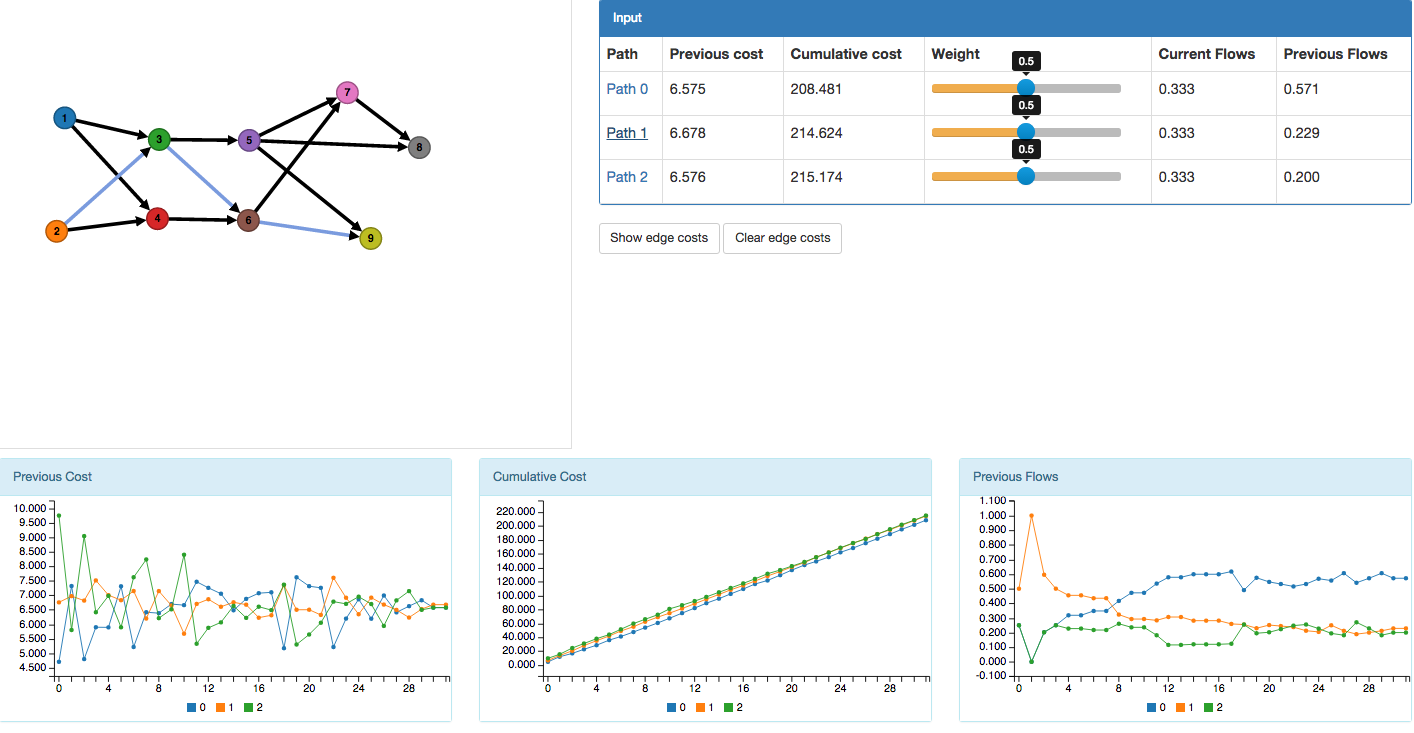
\includegraphics[width=160mm]{images/user_interface}
  \caption{Web interface for the routing game.}
  \label{fig:web_interface}
\end{figure*}


%-----------------------------------------------------------------------------------------------------------------------------------------------------------------
\subsection{Convergence}

To address a player who may be at a disadvantage due to having longer paths or more congested paths because of the topology of the network, we normalized the cumulative path cost of each player with their cumulative path cost at equilibrium. We calculate this equilibrium path cost with Algorithm~\ref{alg:MD}.

At the beginning of the game, there is a clear exploration phase where players tend make aggressive assignments with their flow distribution. Towards the end of the game, the players consolidate their position and make more conservative flow distribution assignments, as seen with Figure~\ref{fig:normalized_costs}.

We can further show this consolidation from the players by computing the Rosenthal potential for the game. As the game progresses, we can see that the Rosenthal potential approaches the optimal value as seen in Figure~\ref{fig:global_potential}.

\begin{figure}
  \centering
  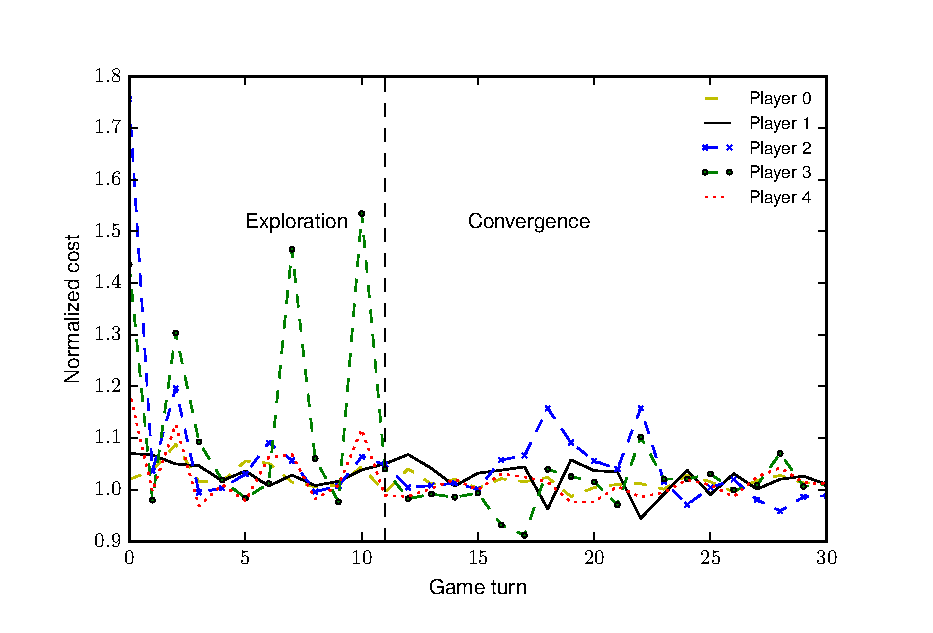
\includegraphics[width=80mm]{images/players_costs}
  \caption{Player normalized cost.}
  \label{fig:normalized_costs}
\end{figure}

\begin{figure}
  \centering
  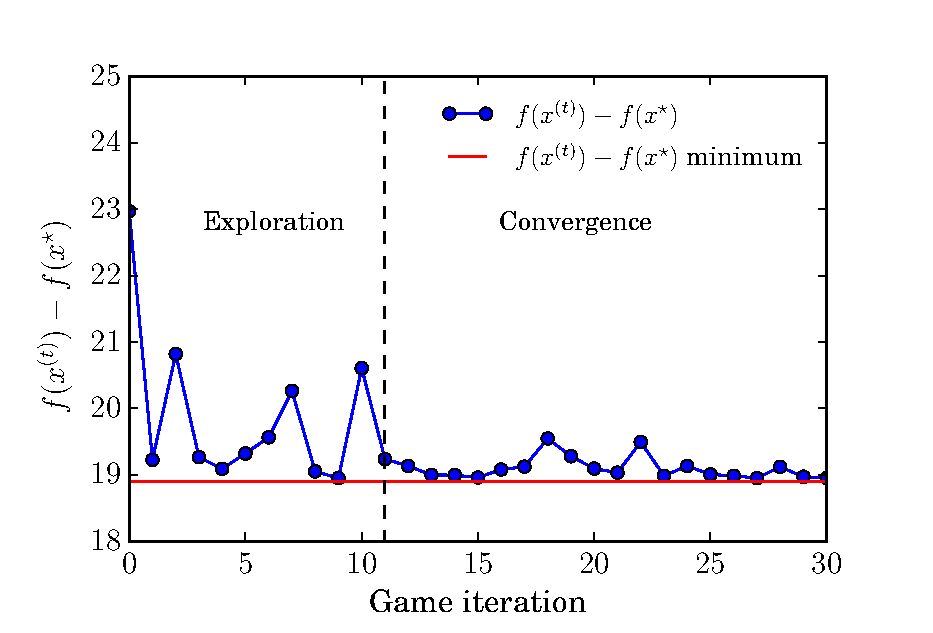
\includegraphics[width=80mm]{images/global_potential_function}
  \caption{Rosenthal potential of the game.}
  \label{fig:global_potential}
\end{figure}

\subsection{Estimation and prediction}

We can estimate the learning rate of each player with the update in \ref{eq:estimation_eta}. We can see that the learning rates of some players are negative at certain turns, which may be explained by the players assuming a contrarian play style at flow distribution assignments for those certain turns.

\begin{figure}
  \centering
  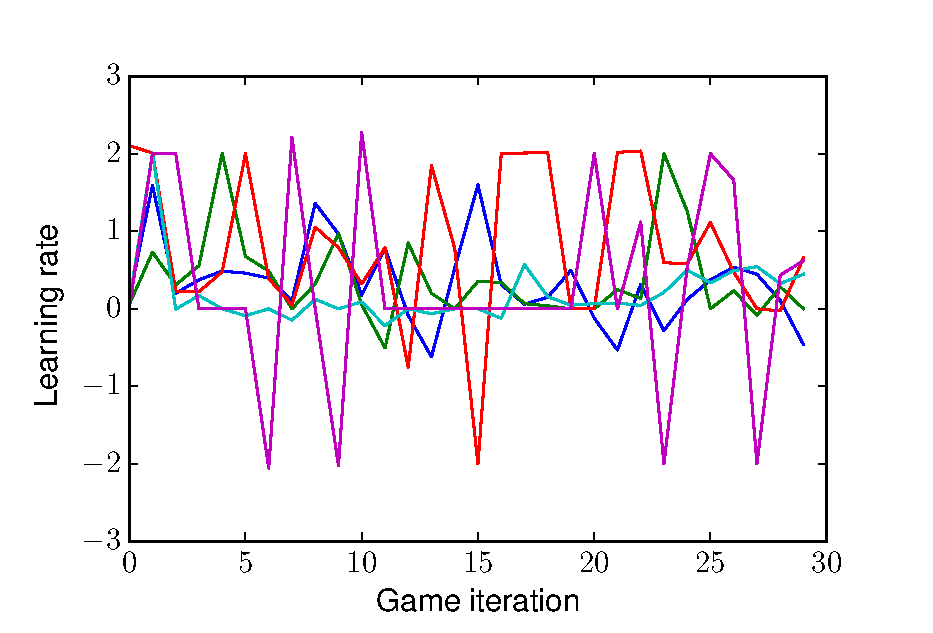
\includegraphics[width=80mm]{images/learning_rate}
  \caption{Learning rate for each player.}
  \label{fig:learning_rates}
\end{figure}

With these estimated sequence of learning rates for each player, we can predict the flow distribution at turn $t+1$ with the learning rate $\eta_t$. We propose three methods for calculating $\eta_t$: first we let $\eta_t=\eta_{t-1}$, second we compute a moving average
\[
\eta_t=\dfrac{1}{N}\sum_{i=t-N-1}^{t-1}\eta_i
\] and finally we compute $\eta_t$ as a linear regression from $\eta_i,\ i \in [0,\ t-1]$.

We also compare these methods with a parameterized sequence of learning rate in Section 3.2

\begin{figure}
  \centering
  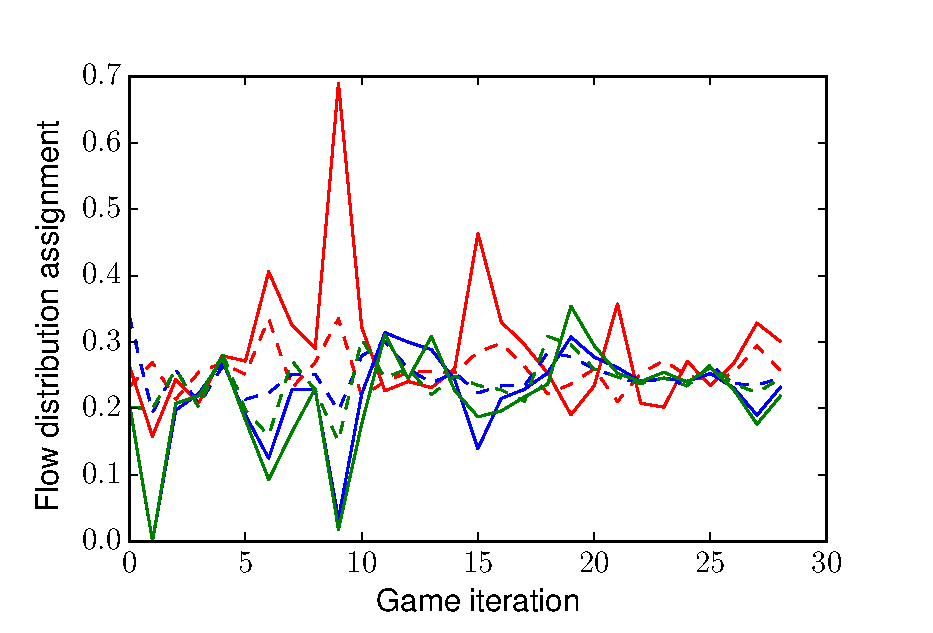
\includegraphics[width=80mm]{images/previous_eta_predictions}
  \caption{Flow distribution predictions $\eta_t = \eta_{t-1}$.}
  \label{fig:previous_eta_predictions}
\end{figure}


\begin{figure}
  \centering
  % \includegraphics[width=80mm]{images/fill_me}
  \missingfigure[figwidth=6cm]{Testing a long text string}
  \caption{Flow distribution predictions moving average $\eta_t$.}
  \label{fig:moving_eta_predictions}
\end{figure}


\begin{figure}
  \centering
  % \includegraphics[width=80mm]{images/fill_me}
  \missingfigure[figwidth=6cm]{Testing a long text string}
  \caption{Flow distribution predictions linear regression $\eta_t$.}
  \label{fig:linear_regression_eta_predictions}
\end{figure}

\begin{figure}
  \centering
  % \includegraphics[width=80mm]{images/fill_me}
  \missingfigure[figwidth=6cm]{Testing a long text string}
  \caption{Flow distribution predictions parameterized $\eta_t$.}
  \label{fig:parameterized_eta_predictions}
\end{figure}


% \begin{figure}
%   \centering
%   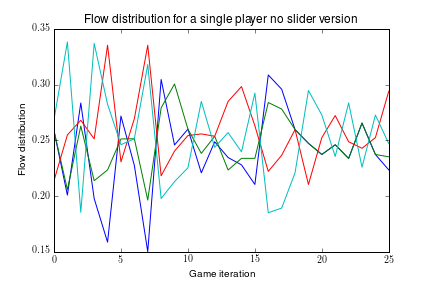
\includegraphics[width=80mm]{images/no_slider_actual_flow_distribution.png}
%   \caption{Player flow distribution.}
%   \label{fig:no_slider_player_flow_distribution}
% \end{figure}

% \begin{figure}
%   \centering
%   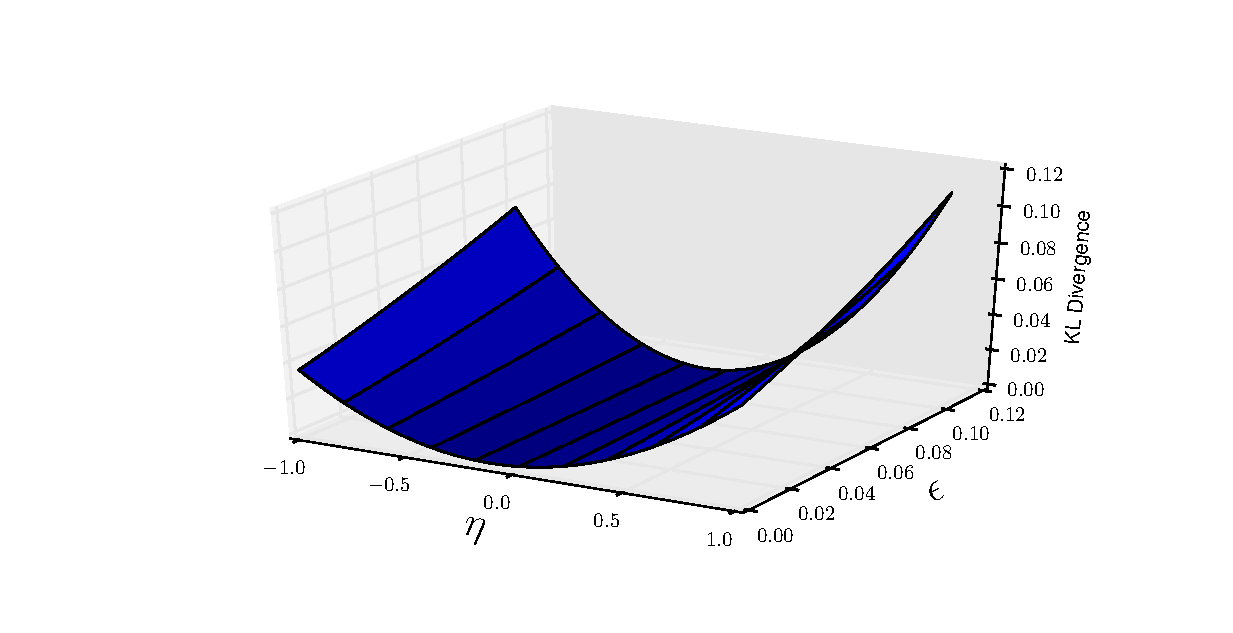
\includegraphics[width=80mm]{images/no_slider_KL_divergence_surface}
%   \caption{KL Divergence surface.}
%   \label{fig:kl_divergence_surface}
% \end{figure}


% \begin{figure}
%   \centering
%   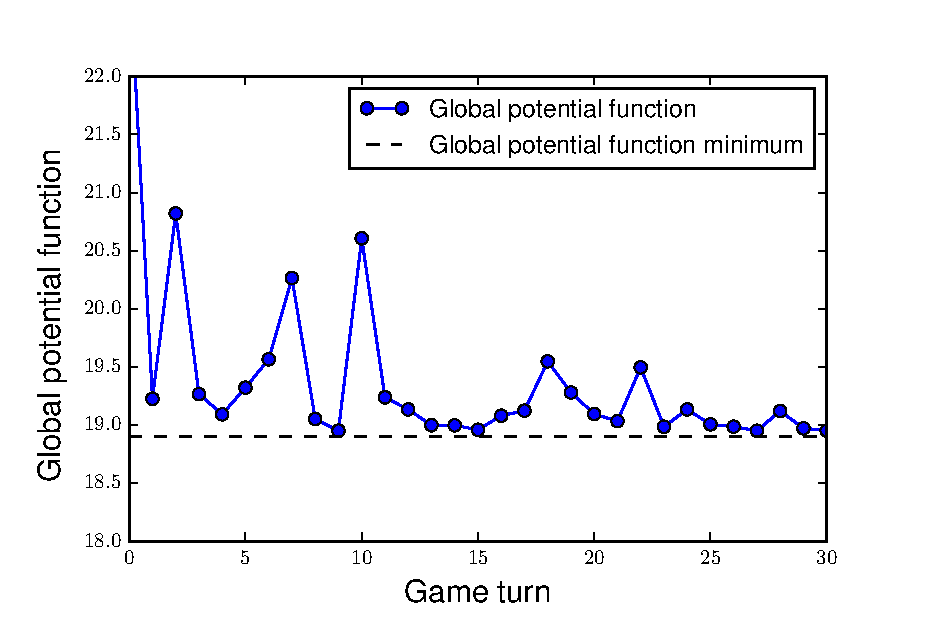
\includegraphics[width=80mm]{images/no_slider_global_potential_function}
%   \caption{Global potential function.}
%   \label{fig:global_potential_function}
% \end{figure}

%-----------------------------------------------------------------------------------------------------------------------------------------------------------------


%============================================================================================
\section{Conclusion}
\label{sec:conclusion}
Conclusion goes here.

%============================================================================================
%ACKNOWLEDGMENTS are optional
\section*{Acknowledgments}
Acknowledgement goes here.

%============================================================================================
%
% The following two commands are all you need in the
% initial runs of your .tex file to
% produce the bibliography for the citations in your paper.
\bibliographystyle{abbrv}
\bibliography{bib}  % sigproc.bib is the name of the Bibliography in this case
% You must have a proper ".bib" file
%  and remember to run:
% latex bibtex latex latex
% to resolve all references
%
% ACM needs 'a single self-contained file'!
%
%APPENDICES are optional
%\balancecolumns
%============================================================================================
\appendix
%Appendix A

Appendix goes here.

% That's all folks!
\end{document}

%%% Local Variables:
%%% mode: latex
%%% TeX-master: t
%%% End:
